\begin{figure*}[t]
\centering
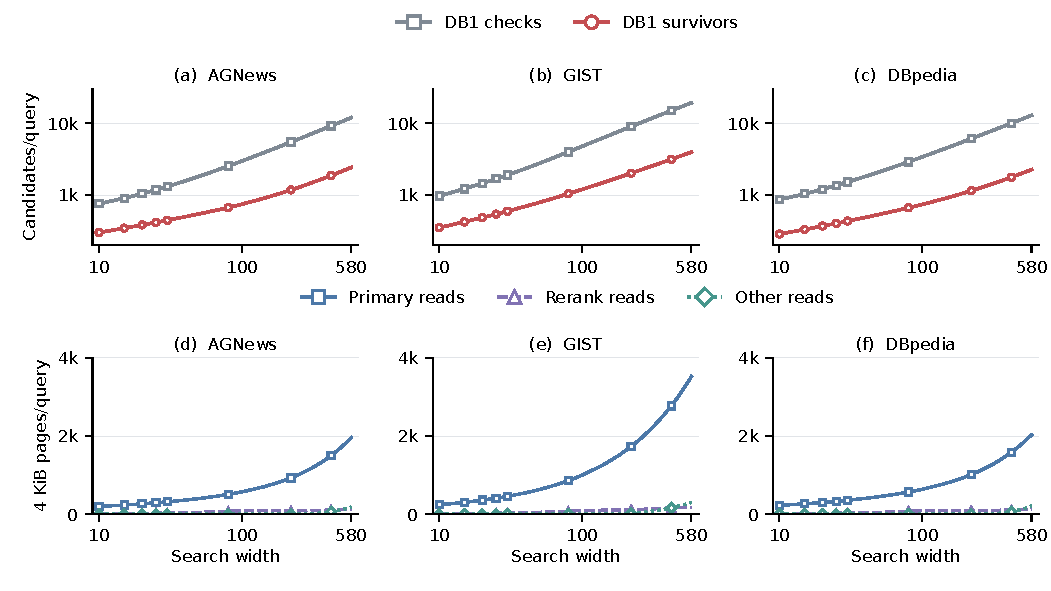
\includegraphics[width=\textwidth]{figures/disk_w32/fig04_screening_io.pdf}
\caption{\textbf{Screening and page demand in the locality variant.} Top: mean DB1 checks and survivors per query, on logarithmic axes. Bottom: mean primary, reranking, and other 4 KiB read pages per query, on a linear vertical scale and logarithmic search-width axis. Other reads equal total read sectors minus primary and reranking pages. These counters do not isolate a causal screening benefit. Measurements use 32 workers and C0 (no cross-query caching), with one run per setting; no between-run uncertainty is estimated.}
\Description{Six panels show screening counts and read-page counts as search width increases on three datasets.}
\label{fig:fig04_screening_io}
\end{figure*}
